\documentclass[a4paper,12pt]{article}
\usepackage[lmargin=30mm,rmargin=30mm,tmargin=25mm,bmargin=25mm]{geometry}
\usepackage[utf8]{inputenc}
\usepackage[T1]{fontenc}
\usepackage{newtxtext} 

\usepackage{textcomp}
\usepackage{fdsymbol}
\usepackage{stmaryrd}
\usepackage{underscore}


\usepackage{newunicodechar}
\newunicodechar{Γ}{$\Gamma$}
\newunicodechar{ε}{$\epsilon$}
\newunicodechar{λ}{$\lambda$}
\newunicodechar{ρ}{$\rho$}
\newunicodechar{σ}{$\sigma$}
\newunicodechar{τ}{$\tau$}
\newunicodechar{∷}{$\Colon$} % requires fdsymbol
%\newunicodechar{∷}{$::$}
\newunicodechar{●}{$\smblkcircle$}
%\newunicodechar{→}{$\rightarrow$} % not needed
\newunicodechar{⇒}{$\Rightarrow$}
\newunicodechar{⟹}{$\Longrightarrow$} % unused
%\newunicodechar{⊹}{$\hermitmatrix$} % requires stix
%\newunicodechar{⊹}{$+$}
\newunicodechar{⊹}{$\Diamond$}
\newunicodechar{⟦}{$\llbracket$}
\newunicodechar{⟧}{$\rrbracket$}
\newunicodechar{⟪}{$\langle\!\langle$}
\newunicodechar{⟫}{$\rangle\!\rangle$}
\newunicodechar{⟨}{$\langle$}
\newunicodechar{⟩}{$\rangle$}
%\newunicodechar{·}{$\cdot$} % not needed
\newunicodechar{⊔}{$\sqcup$}
\newunicodechar{⊓}{$\sqcap$}
\newunicodechar{∈}{$\in$}
%\newunicodechar{¬}{$\neg$} % not needed
\newunicodechar{≡}{$\equiv$}
\newunicodechar{≢}{$\neq$}
\newunicodechar{≤}{$\leq$}
\newunicodechar{≰}{$\nleq$}
\newunicodechar{⊑}{$\sqsubseteq$}
\newunicodechar{ℕ}{$\mathbb{N}$}
\newunicodechar{∘}{$\circ$}
\newunicodechar{₁}{\textsubscript{1}}
\newunicodechar{₂}{\textsubscript{2}}
\newunicodechar{₃}{\textsubscript{3}}
\newunicodechar{η}{$\eta$}
\newunicodechar{⊤}{$\top$}

\usepackage[estonian]{babel}
%\usepackage[none]{hyphenat}


\usepackage{fancyhdr}
\fancypagestyle{FirstPage}{\fancyhf{}\renewcommand{\headrulewidth}{0pt}\fancyfoot[C]{Tallinn 2017}}

\addto\captionsestonian{
  \renewcommand*\contentsname{\centering Sisukord}
  \renewcommand*\listfigurename{\centering Jooniste loetelu}
}

%\usepackage{biblatex}
%\bibliography{thesis}

\usepackage{hyperref}


\usepackage[figure,table]{totalcount}

%\linespread{1.4}
%\renewcommand{\baselinestretch}{1.5}

\setlength{\parindent}{0pt}
\setlength{\parskip}{12pt}

\usepackage{titlesec}

% http://tex.stackexchange.com/questions/299969/titlesec-loss-of-section-numbering-with-the-new-update-2016-03-15
\usepackage{etoolbox}
\makeatletter
\patchcmd{\ttlh@hang}{\parindent\z@}{\parindent\z@\leavevmode}{}{}
\patchcmd{\ttlh@hang}{\noindent}{}{}{}
\makeatother

%\titleformat{\section}[block]{\color{blue}\Large\bfseries\filcenter}{}{1em}{}
\titlespacing*{\section}{0pt}{60pt}{18pt}
\titlespacing*{\subsection}{0pt}{24pt}{12pt}
% III tase: kiri 14pt, lõiguvahe enne ja pärast 12pt

\usepackage{float}
%\floatstyle{boxed} 
%\restylefloat{figure}

\usepackage{fancyvrb}
\fvset{fontsize=\small}
% https://tex.stackexchange.com/questions/2651/should-i-use-center-or-centering-for-figures-and-tables
\makeatletter
\g@addto@macro\@floatboxreset\centering
\makeatother

\usepackage{flafter}

\usepackage{tikz}

\renewcommand{\labelitemi}{$\smblksquare$}

\usepackage{xcolor}
\usepackage[colorinlistoftodos]{todonotes}

\usepackage{setspace}

\begin{document}
\onehalfspacing

\iffalse
\begin{BVerbatim}
λ ⟦ ⟧ ⟪ ⟫ ⟨ ⟩ · ⊹ ∷ ⊔ ⊓ Γ ρ ε σ τ η ∈ ¬ ≡ ≢ ≤ ≰ ⊑ ● → ⇒ ⟹ _ ℕ 
∘ ₁ ₂ ₃ ⊤
\end{BVerbatim}
\fi
% ------------------------------------------------------------
  \begin{center}
    \uppercase{Tallinna Tehnikaülikool}\\
    Infotehnoloogia teaduskond\\
    Tarkvarateaduse instituut\\
    \vfill
    
    Tõnn Talvik 132619IAPM
    \vskip 3em 
    \LARGE\uppercase{efektianalüüsidel põhinevate programmiteisenduste sertifitseerimine}\\
    \normalsize\vskip 4em 
    Magistritöö\\
    \vskip 4em    
  \end{center}
  
  \begin{flushright}
    \begin{tabular}{ r l }
      Juhendaja:& Tarmo Uustalu\\
      & Professor \\
    \end{tabular}
    \vfill
  \end{flushright}
  
  \thispagestyle{FirstPage}
  \clearpage\vspace*{0pt}
  \setcounter{page}{2}
% ------------------------------------------------------------

\section*{\centering Autorideklaratsioon}

Kinnitan, et olen koostanud antud lõputöö iseseisvalt ning seda ei ole kellegi teise poolt varem kaitsmisele esitatud. Kõik töö koostamisel kasutatud teiste autorite tööd, olulised seisukohad, kirjandusallikatest ja mujalt pärinevad andmed on töös viidatud.

Autor: Tõnn Talvik

8. mai 2017

\clearpage\vspace*{0pt}

\section*{\centering Annotatsioon}
[tekst]
         
Lõputöö on kirjutatud eesti keeles ning sisaldab teksti [lehekülgede arv töö põhiosas] leheküljel, [peatükkide arv] peatükki, \totalfigures\ joonist, [tabelite arv] tabelit.
\clearpage\vspace*{0pt}

\section*{\centering Abstract\\
Certification of effect-analysis based program~transformations}

[text]
The thesis is in Estonian and contains [pages] pages of text, [chapters] chapters, \totalfigures\ figures, [tables] tables.
\clearpage\vspace*{0pt}

\tableofcontents
\clearpage\vspace*{0pt}

\listoffigures
\clearpage\vspace*{0pt}



\section{Sissejuhatus}

% background and motivation?
Motivatsioon. Taust: efektid ja monaadid. Moggi, Benton, Katsumata.

Efektisüsteemid on staatilised programmi analüüsid, mis hindavad arvutuste võimalikke efekte.
See võimaldab mh viia läbi optimeerivaid programmiteisendusi.
% https://courses.cs.ttu.ee/pages/Problem_Statement

% Sissejuhatuses tutvustab autor töö teemat, töö eesmärke, lahendatavat probleemistikku,
% andes samuti ülevaate töö ülesehitusest. Sissejuhatuses kirjeldatakse ka töö
% lähtetingimused, alamülesanded ja vajadusel ka täiendavad nõuded (vt jaotist 2.4 ).

% Lõputöös peab sisalduma selge lõpetaja poolt lahendatava ülesande püstitus.

% Magistritöös esitatakse lahendatava ülesande püstitus töö sissejuhatuses, kattes järgmised punktid:
% - töös lahendatavad küsimused ja lähtetingimused,
% - eritingimused, mida on rakendatud ülesande lahendamisel/ülesande püstitamisel.

% Rigor
Agda on sõltuvate tüüpidega funktsionaalne programmeerimiskeel ja interaktiivne tõestusassistent,
mis põhineb intuitsionistlikul tüübiteoorial.
Selles kirjutatud programm on tõlgendatav ja automaatselt kontrollitav kui matemaatiline tõestus.

% Goal
Selle töö eesmärgiks on realiseerida programmeerimiskeeles Agda idee tõendamise
raamistu efektide analüüsiks ja nendele põhinevateks programmiteisendusteks.
Samas raamistus peab saama näidata, et need analüüsid ja teisendused on korrektsed.

Agda on eksperimentaalne keel ja sedalaadi ülesande realisatsioon selles keeles on uudne.
Uurimuse käigus tahame teada, kas niisugune töö on teostatav mõistliku vaevaga, kui õppimisele kuluv aeg maha arvata.

Teoreetilisel tasemel on uudne, et efektide analüüsid ja optimisatsioonid toimivad keele juures, mis toetab andmetüüpe, milleks antud töös on naturaalarvud. \todo{???}

Teises peatükis realiseeritakse näitekeel, mille efektiks on erandid.
Järgmiseks defineeritakse selliste efektide hindamine.
Seejärel arendatakse näitekeelele tüübisüsteem, mille käigus rafineeritakse keelt lisades selle arvutustele efektid ja tüübid.
Edasi antakse rafineeritud keele semantika ning tuuakse mõningased programmiteisendused, näidates, et semantiliselt on tulemus sama.

Kolmandaks peatükis tuuakse efektianalüüs ja optimeerimise näited mitte-determinismi toetava keele kohta.

% Reproducibility
Töö käigus valminud lähtekood on tulemuste reprodutseerimiseks allalaetav aadressilt \url{https://github.com/tonn-talvik/msc}.
Lähtekoodi kompileerimiseks on kasutatud Agda versiooni 2.5.1.1 koos standardteegi versiooniga 0.12.
Mainitud tarkvarapaketid on tasuta installeeritavad Ubuntu 16.04 LTS või teistest varamutest.

\clearpage\vspace*{0pt}

\section{Erandid}

Selles peatükis vaadeldakse keele laiendust eranditega. 
Baaskeeleks on tüübitud lambda-arvutus koos tõeväärtuste, naturaalarvude ja korrutistega.
Järgnevates alapeatükkides defineeritakse selline keel Agdas,
viiakse läbi tüübituletus koos efektianalüüsiga,
määratakse hästi tüübitud avaldiste semantika
ning tuuakse mõned optimeerivate programmiteisenduste näited.
Ühtlasi näidatakse analüüsi ja teisenduste korrektsust.

\subsection{Eranditega keel}\label{ssec:exc.raw}

Vastastikku defineeritud väärtus- ja arvutustüübid on toodud joonisel~\ref{fig:exc.types}.
Lubatud väärtustüübid {\tt VType} on naturaalarvud, tõeväärtused, teiste väärtustüüpide korrutised ja tüübitud lambda-arvutused.
Arvutustüüpideks on efektiga {\tt E} annoteeritud väärtustüübid. Efekt {\tt E} on defineeritud alapeatükis~\ref{sssec:exc.exc}.
\begin{figure}
  \begin{BVerbatim}
mutual
  data VType : Set where
    nat : VType
    bool : VType
    _●_ : VType → VType → VType
    _⇒_ : VType → CType → VType

  data CType : Set where
    _/_ : E → VType → CType
  \end{BVerbatim}
  \caption{Eranditega keele tüübid.}
  \label{fig:exc.types}
\end{figure}


Vastastikku defineeritud väärtus- ja arvutustermid on toodud joonisel~\ref{fig:exc.raw}.
% pragmatics
Termidee konstruktorite nimetamisel on kasutatud suurtähti vältimaks võimalikke nimekonflikte Agda standardfunktsioonidega.
Järgnevalt on selgitatud väärtustermi {\tt vTerm} konstruktorite tähendust.
\begin{itemize}
\item {\tt TT} ja {\tt FF} koostavad vastavalt tõeväärtused tõene ja väär.
\item {\tt ZZ} koostab naturaalarvu 0 ja konstruktor {\tt SS} oma argumendist järgneva naturaalarvu.
\item {\tt ⟨_,_⟩} koostab oma argumentide paari e. korrutise.
\item {\tt FST} ja {\tt SND} koostavad vastavalt argumendina antud korrutise esimese ja teise projektsiooni.
\item {\tt VAR} koostab De~Bruijn'i indeksiga määratud muutuja.
\item {\tt LAM} on funktsiooni abstraktsioon, seejuures funktsiooni parameetri väärtustüüp on eksplitsiitselt annoteeritud. Funktsiooni kehaks on arvutusterm.
\end{itemize}
\begin{figure}
  \begin{BVerbatim}
mutual
  data vTerm : Set where
    TT FF : vTerm
    ZZ : vTerm
    SS : vTerm → vTerm
    ⟨_,_⟩ : vTerm → vTerm → vTerm
    FST SND : vTerm → vTerm
    VAR : ℕ → vTerm
    LAM : VType → cTerm → vTerm

  data cTerm : Set where
    VAL : vTerm → cTerm
    FAIL : VType → cTerm
    TRY_WITH_ : cTerm → cTerm → cTerm
    IF_THEN_ELSE_ : vTerm → cTerm → cTerm → cTerm
    _$_ : vTerm → vTerm → cTerm
    PREC : vTerm → cTerm → cTerm → cTerm
    LET_IN_ : cTerm → cTerm → cTerm
  \end{BVerbatim}
  \caption{Eranditega keele väärtus- ja arvutustermid.}
  \label{fig:exc.raw}
\end{figure}

Järgnevalt on selgitatud arvutustermi {\tt cTerm} konstruktorite (jn~\ref{fig:exc.raw}) tähendust ja vastavas arvutuses kätketud efekti.
\begin{itemize}
\item {\tt VAL} tähistab õnnestunud arvutust, seejuures arvutuse tulemuseks on väärtustermiga antud konstruktori argument.
\item {\tt FAIL} tähistab arvutuse, mille väärtustüüp on eksplitsiitselt annoteeritud, ebaõnnestumist.
\item {\tt TRY_WITH_} on erandikäsitlejaga arvutus: kogu arvutuse tulemuseks on esimese argumendiga antud termi arvutus, kui see õnnestub, vastasel korral aga teise argumendiga antud termi arvutus.
\item {\tt IF_THEN_ELSE_} on valikuline arvutus: vastavalt väärtustermi tõeväärtusele on tulemuseks kas esimese (tõene haru) või teise (väär haru) arvutustermiga antud arvutus.
\item {\tt _\$_} on esimese väärtustermiga antud funktsiooni rakendamine teise väärtustermiga antud väärtusele, kusjuures rakendamise efektiks on funktsioonis peituv efekt.
\item {\tt PREC} on primitiivne rekursioon, mille sammude arv on määratud väärtustermi argumendiga. Esimene arvutusterm vastab rekursiooni baasile ja teine sammule, kusjuures sammuks on akumulaatori ja sammuloenduri parameetritega funktsioon. Kogu arvutuse efekt vastab kõigi osaarvutuste järjestikku sooritamisele.
\item {\tt LET_IN_} lisab esimese arvutustermiga antud väärtuse teise arvutustermi kontekstis esimeseks muutujaks. Arvutuse efekt vastab osaarvutuste järjestikku sooritamisele.
\end{itemize}

\begin{figure}
  \begin{BVerbatim}
ADD : vTerm
ADD = LAM nat
          (VAL (LAM nat
                    (PREC (VAR 0)
                          (VAL (VAR 1))
                          (VAL (SS (VAR 0))))))

ADD-3-and-4 : cTerm
ADD-3-and-4 = LET ADD $ (SS (SS (SS ZZ)))
              IN VAR 0 $ (SS (SS (SS (SS ZZ))))

BAD-ONE : cTerm
BAD-ONE = ZZ $ TT
  \end{BVerbatim}
  \caption{Näidisavaldised eranditega keeles.}
  \label{fig:exc.raw.ex1}
\end{figure}

Joonisel~\ref{fig:exc.raw.ex1} on toodud kahe naturaalarvu liitmise funktsioon väärtustermina {\tt ADD}
ning naturaalarvude 3 ja 4 liitmine arvutustermina {\tt ADD-3-and-4}.
Lisaks on toodud näide arvutustermist {\tt BAD-ONE}, mida annab konstrueerida,
kuid mis ei oma sisu: naturaalarvu null ei saa rakendada tõeväärtusele tõene.
Sellised halvasti tüübitud termid tuvastatakse tüübituletusega (alaptk~\ref{ssec:exc.inference}).

\subsection{Erandite gradeering}\label{ssec:exc.grading}

Selles alapeatükis defineeritakse erandite efekti hinnangud, operatsioonid hinnangutel ja hinnangute omavaheline järjestus.
Sellega võimaldatakse alamtüüpide koostamine.
Ühtlasi näidatakse, et selline hindamine rahuldab eeljärjestatud monoidi ja gradeeritud monaadi omadusi,
millele tuginevad semantika (alaptk~\ref{ssec:exc.semantics}) ja optimisatsioonid (alaptk~\ref{ssec:exc.optimizations}). 

\subsubsection{Erandite efekti hinnang}\label{sssec:exc.exc}

Erandite efekti hinnang {\tt Exc} on toodud joonisel~\ref{fig:exc.exc}:
konstruktor {\tt err} vastab arvutuse ebaõnnestumisele,
konstruktor {\tt ok} arvutuse õnnestumisele ja konstruktor {\tt errok} arvutusele,
mille kohta pole teada, kas see õnnestub või mitte.

\begin{figure}
  \begin{BVerbatim}
data Exc : Set where
  err : Exc
  ok : Exc
  errok : Exc

_·_ : Exc → Exc → Exc
ok · e = e
err · e = err
errok · err = err
errok · ok = errok
errok · errok = errok

_⊹_ : Exc → Exc → Exc
err ⊹ e' = e'
ok ⊹ _ = ok
errok ⊹ ok = ok
errok ⊹ _ = errok
  \end{BVerbatim}
  \caption{Erandite efektid ja operatsioonid nendel.}
  \label{fig:exc.exc}
\end{figure}

Efektide korrutamine {\tt _·_} (jn~\ref{fig:exc.exc}) vastab arvutuste järjestikule sooritamisele.
Kui esimene osaarvutus õnnestub, siis kogu arvutuse efekt on määratud teise osaarvutuse efektiga.
Kui üks osaarvutustest ebaõnnestub, siis ebaõnnestub kogu arvutus.
Ülejäänud juhtudel puudub teadmine arvutuse õnnestumisest või ebaõnnestumisest.
Efektide korrutamine leiab aset {\tt LET_IN_} arvutuses (alaptk~\ref{ssec:exc.raw}).

Erandikäsitleja võib parandada kogu arvutuse hinnangut.
Põhiarvutuse ja erandikäsitleja efeki kombineerimine {\tt _⊹_} on defineeritud joonisel~\ref{fig:exc.exc}.
Kui põhiarvutus ebaõnnestub, siis on kogu arvutuse efekt määratud erandikäsitleja efektiga.
Põhiarvutuse õnnestumisel on kogu arvutus õnnestunud ja erandikäsitlejat ei arvutata.
Kui põhiarvutuse õnnestumine pole teada, aga erandikäsitleja kindlasti õnnestub, siis õnnestub ka kogu arvutus.
Ülejäänud juhtudel pole teada, kas kogu arvutus tervikuna õnnestub või mitte.
Efekti hinnangu parandus leiab aset {\tt TRY_WITH_} arvutuses (alaptk~\ref{ssec:exc.raw}).

Hinnangu {\tt Exc} konstruktorid moodustavad järgneva võre:
\begin{center}
  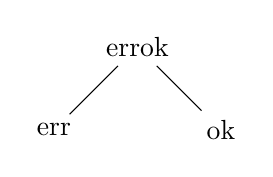
\begin{tikzpicture}[node distance=1.5cm]
    \node (top) at (0,0) {errok};
    \node [below left  of=top] (left)  {err};
    \node [below right of=top] (right) {ok};
    \draw (top) -- (left);
    \draw (top) -- (right);
  \end{tikzpicture}
\end{center}
Hinnangute osaline järjestusseos {\tt _⊑_} on toodud joonisel~\ref{fig:exc.ord}.
See seos on refleksiivne {\tt ⊑-refl}.
Transitiivsuse {\tt ⊑-trans} tõestus seisneb argumentide kuju juhtumi analüüsil.
Transitiivsuse seost on võimalik kodeerida järjestusseose konstruktorina, kuid see pole otstarbekas,
kuna hilisemates tõestuses tekib sellest täiendavad juhtumid, mida peab analüüsima.

\begin{figure}
  \begin{BVerbatim}
data _⊑_ : Exc → Exc → Set where
  ⊑-refl : {e : Exc} → e ⊑ e
  err⊑errok : err ⊑ errok
  ok⊑errok : ok ⊑ errok
  
⊑-trans : {e e' e'' : Exc} → e ⊑ e' → e' ⊑ e'' → e ⊑ e''
⊑-trans ⊑-refl q = q
⊑-trans err⊑errok ⊑-refl = err⊑errok
⊑-trans ok⊑errok ⊑-refl = ok⊑errok

_⊔_ : Exc → Exc → Exc
_⊓_ : Exc → Exc → Maybe Exc
⊔-sym : (e e' : Exc) → e ⊔ e' ≡ e' ⊔ e
⊓-sym : (e e' : Exc) → e ⊓ e' ≡ e' ⊓ e

lub : (e e' : Exc) → e ⊑ (e ⊔ e')
glb : (e e' : Exc) {e'' : Exc} → e ⊓ e' ≡ just e'' → e'' ⊑ e
lub-sym : (e e' : Exc) → e ⊑ (e' ⊔ e)
  \end{BVerbatim}
  \caption{Erandite efektide järjestus.}
  \label{fig:exc.ord}
\end{figure}
Loomulikul viisil saab defineerida erandi hinnangu ülemise ja alumise raja ning näidata nende sümmeetrilisust.
Lihtsuse huvides on toodud ainult vastavad tüübisignatuurid, aga mitte definitsioonid (jn~\ref{fig:exc.ord}).
Kuna kahel hinnangul ei pruugi leiduda alumine raja, siis on {\tt _⊓_} tulemus mähitud {\tt Maybe} monaadi.

\subsubsection{Eeljärjestatud monoid}
Hulk {\tt E}, millel on defineeritud korrutamine {\tt _·_} ja ühikelement {\tt i},
st {\tt i} on ühik korrutamise suhtes nii vasakult {\tt lu} kui ka paremalt {\tt ru},
ning korrutamine on assotsiatiivne {\tt ass}, nimetatakse monoidiks.
Kui sellel hulgal on osaline järjestusseos {\tt _⊑_},
mis on refleksiivne {\tt ⊑-refl} ja transitiivne {\tt ⊑-trans},
ning kehtib korrutamise monotoonsus {\tt mon},
siis on tegemist eeljärjestatud monoidiga.
Joonisel~\ref{fig:ordered-monoid} on toodud eeljärjestatud monoidi kirje tüüp Agdas.

\begin{figure}
  \begin{BVerbatim}
record OrderedMonoid : Set where
  field
    E : Set
    _·_ : E → E → E    
    i : E

    lu : {e : E } → i · e ≡ e
    ru : {e : E } → e ≡ e · i 
    ass : {e e' e'' : E} → (e · e') · e'' ≡ e · (e' · e'')
    
    _⊑_ : E → E → Set    
    ⊑-refl : {e : E} → e ⊑ e
    ⊑-trans : {e e' e'' : E} → e ⊑ e' → e' ⊑ e'' → e ⊑ e''

    mon : {e e' e'' e''' : E} → e ⊑ e'' → e' ⊑ e''' → e · e' ⊑ e'' · e'''
  \end{BVerbatim}
  \caption{Eeljärjestatud monoid.}
  \label{fig:ordered-monoid}
\end{figure}

Saab näidata, et erandite hinnag {\tt Exc},
korrutamine {\tt _·_}, mille ühikuks on konstruktor {\tt ok},
ja osaline järjestusseos {\tt _⊑_} moodustavad eeljärjestatud monoidi instantsi.
Vasakühiku tõestus tuleneb vahetult korrutamise definitsioonist.
Paremühiku tõestamisel tuleb teha juhtumi analüüs varjatud argumendi konstruktori kuju peal
ja seejärel lähtuda korrutamise definitsioonist.
Assotsiatiivsus tõestatakse sarnaselt kasutades juhtumite analüüsi ja korrutamise definitsiooni. Monotoonsuse tõestuses analüüsitakse nii võimalikke efekte kui ka nendevahelisi järjestusseoseid.
Kõik mainitud tõestused on toodud töö käigus valminud lähtekoodis.


\subsubsection{Gradeeritud monaad}

Efektiga {\tt E} parametriseeritud tüübikonstruktor {\tt T} koos tagastamisega {\tt η} ja sidumisega {\tt bind}  moodustab monaadi.
Neelduvus {\tt sub} on refleksiivne {\tt sub-refl}, transitiivne {\tt sub-trans} ja  sidumise suhtes monotoonne {\tt sub-mon}.
Täidetud on monaadi seadused {\tt mlaw1}, {\tt mlaw2} ja {\tt mlaw3}.

Joonisel~\ref{fig:graded-monad} on toodud gradeeritud monaadi kirje tüüp Agdas.

\begin{figure}
  \begin{BVerbatim}
subeq : {E : Set} → {T : E → Set → Set} → {e e' : E} → {X : Set} →
        e ≡ e' → T e X → T e' X
subeq refl p = p


record GradedMonad : Set where
  field
    OM : OrderedMonoid
  open OrderedMonoid OM
  field

    T : E → Set → Set
    η : {X : Set} → X → T i X
    bind : {e e' : E} {X Y : Set} → (X → T e' Y) → (T e X → T (e · e') Y)

    sub : {e e' : E} {X : Set} → e ⊑ e' → T e X → T e' X

    sub-mon : {e e' e'' e''' : E} {X Y : Set} →
              (p : e ⊑ e'') → (q : e' ⊑ e''') → 
              (f : X → T e' Y) → (c : T e X) → 
              sub (mon p q) (bind f c) ≡ bind (sub q ∘ f) (sub p c) 

  sub-eq : {e e' : E} {X : Set} → e ≡ e' → T e X → T e' X
  sub-eq = subeq {E} {T}
 
  field
    sub-refl : {e : E} {X : Set} → (c : T e X) → sub ⊑-refl c ≡ c
    sub-trans : {e e' e'' : E} {X : Set} →
                (p : e ⊑ e') → (q : e' ⊑ e'') → (c : T e X) → 
                sub q (sub p c) ≡ sub (⊑-trans p q) c   

    mlaw1 : {e : E} → {X Y : Set} → (f : X → T e Y) → (x : X) →
            sub-eq lu (bind f (η x)) ≡ f x
    mlaw2 : {e : E} → {X : Set} → (c : T e X) →
            sub-eq ru c ≡ bind η c
    mlaw3 : {e e' e'' : E} → {X Y Z : Set} →
            (f : X → T e' Y) → (g : Y → T e'' Z) → (c : T e X) → 
            sub-eq ass (bind g (bind f c)) ≡ bind (bind g ∘ f) c 

  T₁ : {e : E} {X Y : Set} → (X → Y) → T e X → T e Y
  T₁ f = sub-eq (sym ru) ∘ bind (η ∘ f)
  \end{BVerbatim}
  \caption{Gradeeritud monaad.}
  \label{fig:graded-monad}
\end{figure}

Saab näidata, et erandite järjestatud monoidil saab põhineda gradeeritud monaad.

\subsection{Tüübi- ja efektituletus} \label{ssec:exc.inference}

\subsubsection{Alamtüübid}
Väärtus- ja arvutustüüpide osaline järjestatus on vastastikku defineeritud (jn~\ref{fig:exc.subtypes}).
Konstruktoriga {\tt st-bn} loetakse tõeväärtused naturaalarvude alamtüübiks.
Kehtib väärtustüüpide refleksiivsus {\tt st-refl}.
Üks väärtustüübi paar on teise alamtüüp {\tt st-prod}, kui paaride vastavad projektsioonid on omakorda alamtüübid.
Funktsioonid on alamtüübid {\tt st-func}, kui funktsioonide kehade arvutused on alamtüübid,
ja funktsioonide argumendid on kontravariantsed.
Arvutustüüp on teise arvutustüübi alamtüüp {\tt st-comp}, kui nende efektid ja väärtustüübid on järjestatud.
\begin{figure}
  \begin{BVerbatim}
mutual
  data _≤V_ : VType → VType → Set where
    st-bn : bool ≤V nat
    st-refl : {σ : VType} → σ ≤V σ
    st-prod : {σ σ' τ τ' : VType} →
              σ ≤V σ' → τ ≤V τ' → σ ● τ ≤V σ' ● τ'
    st-func : {σ σ' : VType} {τ τ' : CType} →
              σ' ≤V σ → τ ≤C τ' → σ ⇒ τ ≤V σ' ⇒ τ'

  data _≤C_ : CType → CType → Set where
    st-comp : {e e' : E} {σ σ' : VType} →
              e ⊑ e' → σ ≤V σ' → e / σ ≤C e' / σ'

mutual
  st-trans : {σ σ' σ'' : VType} → σ ≤V σ' → σ' ≤V σ'' → σ ≤V σ''
  st-trans st-refl q = q
  st-trans p st-refl = p
  st-trans (st-prod p p') (st-prod q q') = st-prod (st-trans p q)
                                                   (st-trans p' q')
  st-trans (st-func p p') (st-func q q') = st-func (st-trans q p)
                                                   (sct-trans p' q')

  sct-trans : {σ σ' σ'' : CType} → σ ≤C σ' → σ' ≤C σ'' → σ ≤C σ''
  sct-trans (st-comp p q) (st-comp p' q') = st-comp (⊑-trans p p')
                                                    (st-trans q q')
  \end{BVerbatim}
  \caption{Väärtus- ja arvutustüüpide alamtüüpimine.}
  \label{fig:exc.subtypes}
\end{figure}

Väärtus- ja arvutustüüpide alamtüüpide transitiivsus on defineeritud vastastikku joonisel~\ref{fig:exc.subtypes}.
\todo{explain}

\subsubsection{Rafineeritud keel}

Joonisel~\ref{fig:exc.refined} on toodud vastastikku defineeritud rafineeritud väärtus- ja arvutustermid.
Kontekst {\tt Ctx} on defineeritud kui väärtusttüüpide list.
Võrreldes alaptk~\ref{ssec:exc.raw}-s toodud termidega, on rafineeritud termid parametriseeritud kontekstiga {\tt Γ} ning indekseeritud vastavalt väärtus- ja arvutustüüpidega.
\begin{itemize}
\item Konstruktorid {\tt TT} ja {\tt FF} koostavad tõeväärtustüüpi termi.
\item Konstruktor {\tt ZZ} koostab naturaalarvu tüüpi termi. Konstruktor {\tt SS} koostab antud naturaalarvu tüüpi termi järglase, mis on samuti naturaalarvu tüüpi.
\item {\tt ⟨_,_⟩} koostab kahest antud väärtustermist paari, mille tüüp on termide tüüpide korrutis.
\item {\tt FST} ja {\tt SND} projekteerivad paari tüüpi termist vastavalt esimese või teise korrutatava tüüpi termi.
\item {\tt VAR} võtab tõestuse, et mingi tüüp on konteksti element, ning annab väärtustermi, mille tüüp on kõnealuse elemendiga määratud tüüp.
\item {\tt LAM} võtab väärtustüübi ja arvutustermi, mille kontekst on parameetriga antud kontekstist täpselt väärtustüübi argumendi võrra suurem, ning annab funktsiooniruumile vastava väärtustermi.
\item {\tt VCAST} suurendab ettantud väärtustermi tüüpi vastavalt alamtüübi tõestusele. See võimaldab erinevate alamtüüpidega väärtustermid ühtlustada, mis on vajalik rafineeritud arvutustermide koostamisel.
\end{itemize}

\begin{figure}
  \begin{BVerbatim}
Ctx = List VType

mutual
 data VTerm (Γ : Ctx) : VType → Set where
   TT FF : VTerm Γ bool
   ZZ : VTerm Γ nat
   SS : VTerm Γ nat → VTerm Γ nat
   ⟨_,_⟩ : {σ σ' : VType} →
           VTerm Γ σ → VTerm Γ σ' → VTerm Γ (σ ● σ')
   FST : {σ σ' : VType} → VTerm Γ (σ ● σ') → VTerm Γ σ
   SND : {σ σ' : VType} → VTerm Γ (σ ● σ') → VTerm Γ σ'
   VAR : {σ : VType} → σ ∈ Γ → VTerm Γ σ
   LAM : (σ : VType) {τ : CType} →
         CTerm (σ ∷ Γ) τ → VTerm Γ (σ ⇒ τ)
   VCAST : {σ σ' : VType} → VTerm Γ σ → σ ≤V σ' → VTerm Γ σ'

 data CTerm (Γ : Ctx) : CType → Set where
   VAL : {σ : VType} → VTerm Γ σ → CTerm Γ (ok / σ)
   FAIL : (σ : VType) → CTerm Γ (err / σ)
   TRY_WITH_ : {e e' : E} {σ : VType} → CTerm Γ (e / σ) →
               CTerm Γ (e' / σ) → CTerm Γ (e ⊹ e' / σ)
   IF_THEN_ELSE_ : {e e' : E} {σ : VType} → VTerm Γ bool →
                CTerm Γ (e / σ) → CTerm Γ (e' / σ) → CTerm Γ (e ⊔ e' / σ)
   _$_ : {σ : VType} {τ : CType} →
         VTerm Γ (σ ⇒ τ) → VTerm Γ σ → CTerm Γ τ
   PREC : {e e' : E} {σ : VType} → VTerm Γ nat →
          CTerm Γ (e / σ) → CTerm (σ ∷ nat ∷ Γ) (e' / σ) →
          e · e' ⊑ e → CTerm Γ (e / σ)
   LET_IN_ : {e e' : E} {σ σ' : VType} → CTerm Γ (e / σ) →
             CTerm (σ ∷ Γ) (e' / σ') → CTerm Γ (e · e' / σ')
   CCAST : {e e' : E} {σ σ' : VType} → CTerm Γ (e / σ) →
           e / σ ≤C e' / σ' → CTerm Γ (e' / σ')
  \end{BVerbatim}
  \caption{Eranditega keele rafineeritud termid.}
  \label{fig:exc.refined}
\end{figure}

Rafineeritud arvutustermid (jn \ref{fig:exc.refined}) määravad täpselt osaarvutuste efektide kombineerimise.
\begin{itemize}
\item {\tt VAL} koostab antud väärtustermist õnnestunud arvutuse.
\item {\tt FAIL} koostab väärtustüübist ebaõnnestunud arvutuse.
\item {\tt TRY_WITH_} parandab põhiarvutustermi efekti erandikäsitleja arvutustermi efektiga. Kitsendusena peavad arvutustermid omama sama väärtustüüpi.
\item {\tt IF_THEN_ELSE_} eeldab tõeväärtustüüpi tingimust. Kogu arvutustermi efekt on määratud harude, millede väärtustüübid peavad ühtima, efektide ülemise rajaga.
\item {\tt _\$_} rakendab esimesega väärtustermiga antud funktsiooni teise väärtustermiga argumendile, seejuures peavad funktsiooni parameetri ja argumendi väärtustüübid ühtima. Kogu arvutuse efekt ja väärtustüüp on määratud funktsiooni keha arvutustüübiga. 
\item {\tt PREC} eeldab sammude arvuna naturaalarvude tüüpi väärtustermi. Baasarvutuse väärtustüüp on lisatud koos naturaalarvu tüüpi sammuloenduriga sammu arvutustermi konteksti. Täiendava kitsendusena on nõutud, et baasi efekt oleks sammu efektiga korrutamisel püsipunkt.
\item {\tt LET_IN_} lisab esimese arvutustermi väärtustüübi teise arvutustermi konteksti. Kogu arvutuse efektis on arvutustermide korrutis ning väärtustüüp on määratud teise arvutustermi tüübiga.
\item {\tt CCAST} suurendab etteantud arvutustermi tüüpi vastavalt alamtüübi tõestusele.
\end{itemize}


\subsubsection{Termide tüübituletus}\label{sssec:exc.infer-type}

Etteantud kontekstis saab väärtustermile tuletada vastava väärtustüübi (jn \ref{fig:exc.infer-vtype}).
Kuna vaste võib puududa, siis on {\tt infer-vtype} tulemus mähitud {\tt Maybe} monaadi.
Väärtustüübi tuletamisel lähtutakse väärtustüübi konstruktori kujust.
\begin{itemize}
\item {\tt TT} ja {\tt FF} annavad kindlasti tõeväärtustüübi.
\item {\tt ZZ} on kindlasti naturaalarvu tüüpi. {\tt SS t} korral tuleb täiendavalt kontrollida, kas alamterm {\tt t} on samas kontekstis naturaalarvu tüüpi. Vastasel korral on term halvasti koostatud ja selle tüüp puudub.
\item Paari {\tt ⟨ t , t' ⟩} tüüp on määratud, kui alamtermide {\tt t} ja {\tt t'} tüübid on samas kontekstis määratud. Paari tüübiks on alamtermide tüüpide korrutis. Ülejäänud juhtudel pole paari tüüp määratud.
\item {\tt FST t} ja {\tt SND t} on määratud, kui alamterm {\tt t} on paar, st antud kontekstis on ta korrutise tüüpi. Projektsiooni tüübiks on vastavalt esimene või teine korrutatav.
\item {\tt VAR x} korral tuleb kontrollida, et naturaalarv {\tt x} on väiksem kui kontekst {\tt Γ} pikkus. Selleks on kasutatud lahendajat {\tt _<?_}. Naturaalarvude võrratusest {\tt p} on koostatud konteksti pikkusega piiratud naturaalarv {\tt fromℕ≤ p}, mida kasutatakse muutujale vastava tüübi otsimiseks kontekstist {\tt lkp Γ}.
\item {\tt LAM σ t} puhul tuleb kontrollida, et arvutustermiga {\tt t} antud keha on hästi tüübitud kontekstis, mida on laiendatud parameetri {\tt σ} võrra. Arvutustermi tüübituletus {\tt infer-ctype} on toodud allpool.
\end{itemize}

\begin{figure}
  \begin{BVerbatim}
infer-vtype : Ctx → vTerm → Maybe VType
infer-vtype Γ TT = just bool
infer-vtype Γ FF = just bool
infer-vtype Γ ZZ = just nat
infer-vtype Γ (SS t) with  infer-vtype Γ t
... | just nat = just nat
... | _        = nothing
infer-vtype Γ ⟨ t , t' ⟩ with infer-vtype Γ t | infer-vtype Γ t'
... | just σ | just σ' = just (σ ● σ')
... | _      | _       = nothing
infer-vtype Γ (FST t) with infer-vtype Γ t
... | just (σ ● _) = just σ
... | _            = nothing
infer-vtype Γ (SND t) with infer-vtype Γ t
... | just (_ ● σ') = just σ'
... | _             = nothing
infer-vtype Γ (VAR x) with x <? Γ
... | yes p = just (lkp Γ (fromℕ≤ p))
... | no ¬p = nothing
infer-vtype Γ (LAM σ t) with infer-ctype (σ ∷ Γ) t
... | just τ = just (σ ⇒ τ)
... | _      = nothing
  \end{BVerbatim}
  \caption{Eranditega keele väärtustermide tüübituletus.}
  \label{fig:exc.infer-vtype}
\end{figure}

Joonisel \ref{fig:exc.infer-ctype} on toodud etteantud kontekstis arvutustermile tüübi tuletamine.
Nagu väärtustermide tüübituletuse puhul, on ka arvutustermide tüübituletus {\tt infer-ctype} tulemus mähitud {\tt Maybe} monaadi.
Väärtustüübi tuletamisel lähtutakse väärtustüübi konstruktori kujust.
\begin{itemize}
\item {\tt VAL x} on tüübitud, kui väärtustermi {\tt x} tüübituletus õnnestub. Arvutuse väärtustüübiks on tuletatud tüüp. Efekti hinnang {\tt ok} tähistab arvutuse õnnestumist. 
\item {\tt FAIL σ} on alati väärtustüübi {\tt σ} ebaõnnestumise tüüpi, mille efekti hinnang on {\tt err}.
\item {\tt TRY t WITH t'} on tüübitud, kui arvutustermid {\tt t} ja {\tt t'} on hästi tüübitud. Kogu arvutuse tüübiks on põhiarvutuse tüübi {\tt τ} parandamine erandikäsitleja tüübiga {\tt τ'}. Arvutustüüpide parandus _⊹C_ on defineeritud efektide paranduse _⊹_ ja väärtustüüpide ülemise raja _⊔V_ abil.
\item {\tt IF x THEN t ELSE t'} eeldab, et väärtusterm {\tt x} on tõeväärtustüüpi. Kogu arvutuse tüüp on määratud harude tüüpide {\tt τ} ja {\tt τ'} ülemise rajaga {\tt τ ⊔C τ'}.
\item {\tt f \$ t} korral kontrollitakse, et väärtustermi {\tt f} tüübiks on funktsiooniruum ja väärtustermile {\tt t} tuletatud tüüp on {\tt f} parameetri alamtüüp. Ülejäänud juhtudel ei ole funktsiooni rakendamine hästi tüübitud.
\item {\tt PREC x t t'} korral kontollitakse viit tingimust.
  \begin{itemize}
  \item Väärtusterm {\tt x} peab olema antud kontekstis naturaalarvu tüüpi.
  \item Baasi arvutusterm {\tt t} peab olema antud kontekstis hästi tüübitud.
  \item Sammu arvutusterm {\tt t'} peab olema tüübitud kontekstis, kuhu on lisatud naturaalarvu tüübi sammuloendur ja arvutustermi {\tt t} väärtustüüpi {\tt σ} akumulaator.
  \item Osaarvutustele tuletatud väärtustüübid peavad olema samad. Selleks kasutatakse lahendajat {\tt _≡V?_}.
  \item Osaarvutuste efektide korrutis ei tohi olla suurem, kui baasi efekt. Seda kontrollitakse lahendajaga {\tt _⊑?_}.
  \end{itemize}
  Kui kõik tingimused kehtivad, siis kogu arvutuse tüüp on määratud baasi efekti ja väärtustüübiga.
\item {\tt LET t IN t'} on tüübitud, kui arvutusterm {\tt t} on tüübitud antud kontekstis ja arvutusterm {\tt t'} on tüübitud kontekstis, mida on laiendatud esimese osaarvutuse väärtustüübi võrra. Arvutuse efektiks on osarvutuste efektide korrutis ning väärtustüübiks teise osaarvutuse väärtustüüp. Kui üks osaarvutust ei ole hästi tüübitud, siis ei ole ka kogu arvutus tüübitud.
\end{itemize}

\begin{figure}
  \begin{BVerbatim}
infer-ctype : Ctx → cTerm → Maybe CType
infer-ctype Γ (VAL x) with infer-vtype Γ x
... | just σ = just (ok / σ)
... | _      = nothing
infer-ctype Γ (FAIL σ) = just (err / σ)
infer-ctype Γ (TRY t WITH t') with infer-ctype Γ t | infer-ctype Γ t'
... | just τ | just τ' = τ ⊹C τ'
... | _      | _       = nothing
infer-ctype Γ (IF x THEN t ELSE t')
    with infer-vtype Γ x | infer-ctype Γ t | infer-ctype Γ t'
... | just bool | just τ | just τ' = τ ⊔C τ'
... | _         | _      | _       = nothing
infer-ctype Γ (f $ t) with infer-vtype Γ f | infer-vtype Γ t
... | just (σ ⇒ τ) | just σ' with σ' ≤V? σ
...                           | yes _ = just τ
...                           | no  _ = nothing
infer-ctype Γ (f $ t) | _ | _ = nothing
infer-ctype Γ (PREC x t t')
    with infer-vtype Γ x
... | just nat with infer-ctype Γ t
...        | nothing = nothing
...        | just (e / σ) with infer-ctype (σ ∷ nat ∷ Γ) t'
...                       | nothing = nothing
...                       | just (e' / σ') with e · e' ⊑? e | σ ≡V? σ'
...                                        | yes _ | yes _ = just (e / σ)
...                                        | _     | _     = nothing
infer-ctype Γ (PREC x t t') | _ = nothing
infer-ctype Γ (LET t IN t') with infer-ctype Γ t 
... | nothing = nothing
... | just (e / σ) with infer-ctype (σ ∷ Γ) t'
...                | nothing        = nothing
...                | just (e' / σ') = just (e · e' / σ')
  \end{BVerbatim}
  \caption{Eranditega keele arvutustermide tüübituletus.}
  \label{fig:exc.infer-ctype}
\end{figure}

\subsubsection{Termide rafineerimine}

Kui n-ö ``toorele'' termile õnnestub mingis kontekstis tuletada tüüp, siis saab sellest termist konstrueerida rafineeritud termi.
Joonisel \ref{fig:exc.infer-term-type} on toodud väärtus- ja arvutustermide rafineeritud tüübikonstruktorid.
Tipp-tüüp {\tt ⊤} tähistab tüübituletuse ebaõnnestumist.
\begin{figure}
  \begin{BVerbatim}
refined-vterm : Ctx → vTerm → Set
refined-vterm Γ t with infer-vtype Γ t 
... | nothing = ⊤
... | just τ = VTerm Γ τ

refined-cterm : Ctx → cTerm → Set
refined-cterm Γ t with infer-ctype Γ t 
... | nothing = ⊤
... | just τ = CTerm Γ τ
  \end{BVerbatim}
  \caption{Väärtus- ja arvutustermide rafineerimiste tüübikonstruktorid.}
  \label{fig:exc.infer-term-type}
\end{figure}

Väärtustermide rafineerimine etteantud kontekstis (jn \ref{fig:exc.refine-vterm}) matkib väärtustermide tüübituletust (alaptk \ref{sssec:exc.infer-type}).
\begin{itemize}
\item {\tt TT} ja {\tt FF} korral konstrueeritakse vastav rafineeritud väärtusterm.
\item {\tt ZZ} puhul konstrueeritakse rafineeritud väärtusterm null {\tt ZZ}. {\tt SS t} korral kontrollitakse, et väärtusterm {\tt t} on hästi tüübitud ja on naturaalarvu tüüpi. Rafineeritud naturaalarvu järglane {\tt SS} koostatakse alamväärtuse {\tt t} rafineeringust {\tt u}. Kui väärtustermi {\tt t} tüübituletus ei õnnestu või tuletatud tüüp ei ole naturaalarvu tüüpi, siis rafineeringu tulemuseks koostatakse tipp-tüübi element {\tt tt}.
\item {\tt ⟨ t , t' ⟩} korral kontrollitakse, et mõlemad väärtustermid {\tt t} ja {\tt t'} on kontekstis hästi tüübitud ja rafineeritud paar koostatakse rafineeritud termidest {\tt u} ja {\tt u'}.
\item {\tt FST t} puhul peab väärtustermile {\tt t} tuletatud tüüp olema korrutis. Rafineeritud projektsiooni saab koostada {\tt t} rafineeringust {\tt u}. {\tt SND t} juhtum on analoogne.
\item {\tt VAR x} korral koostatakse lahendist {\tt p}, mis näitab, et naturaalarv {\tt x} on väiksem kui konteksti {\tt Γ} pikkus, rafineeritud muutuja tõestusega, et {\tt x}-iga määratud muutuja on kontekstis.
\item {\tt LAM σ t} juhtumis lisatakse parameetri tüüp {\tt σ} konteksti ja kontrollitakse arvutustermi {\tt t} hästi-tüübitust. Rafineeritud funktsiooni abstraktsioon koostatakse uues kontekstis rafineeritud arvutusest {\tt u}.
\end{itemize}

\begin{figure}
  \begin{BVerbatim}
refine-vterm : (Γ : Ctx) (t : vTerm) → refined-vterm Γ t 
refine-vterm Γ TT = TT
refine-vterm Γ FF = FF
refine-vterm Γ ZZ = ZZ
refine-vterm Γ (SS t) with infer-vtype Γ t | refine-vterm Γ t
... | just nat | u = SS u
... | just bool | _ = tt
... | just (_ ● _) | _ = tt
... | just (_ ⇒ _) | _ = tt
... | nothing | _ = tt
refine-vterm Γ ⟨ t , t' ⟩
    with infer-vtype Γ t | refine-vterm Γ t |
         infer-vtype Γ t' | refine-vterm Γ t'
... | just _  | u | just _  | u' = ⟨ u , u' ⟩
... | just _  | _ | nothing | _  = tt
... | nothing | _ | _       | _  = tt
refine-vterm Γ (FST t) with infer-vtype Γ t | refine-vterm Γ t
... | just nat | _ = tt
... | just bool | _ = tt
... | just (_ ● _) | u = FST u
... | just (_ ⇒ _) | _ = tt
... | nothing | _ = tt
refine-vterm Γ (SND t) with infer-vtype Γ t | refine-vterm Γ t
... | just nat | _ = tt
... | just bool | _ = tt
... | just (_ ● _) | u = SND u
... | just (_ ⇒ _) | _ = tt
... | nothing | _ = tt
refine-vterm Γ (VAR x) with x <? Γ
... | yes p = VAR (trace Γ (fromℕ≤ p))
... | no _  = tt
refine-vterm Γ (LAM σ t)
    with infer-ctype (σ ∷ Γ) t | refine-cterm (σ ∷ Γ) t
... | just _ | u = LAM σ u
... | nothing | u = tt
  \end{BVerbatim}
  \caption{Eranditega keele väärtustermide rafineerimine.}
  \label{fig:exc.refine-vterm}
\end{figure}

Arvutustermide rafineerimine on toodud joonistel \ref{fig:exc.refine-cterm1} ja \ref{fig:exc.refine-cterm2}.
\begin{itemize}
\item {\tt VAL t} korral kontrollitakse, et väärtusterm {\tt t} on hästi tüübitud, ja rafineeritud arvutus koostatakse vastavast rafineeritud väärtustermist {\tt u}.
\item {\tt FAIL σ} rafineerimisel näidatakse, et selle arvutustermi tüübituletus alati õnnestub.
\item {\tt TRY t WITH t'} korral kontrollitakse, et mõlemad osaarvutused on hästi tüübitud ja tuletatud väärtustüüpidel leidub ülemine raja. Rafineeritud arvutuse konstrueerimiseks suurendatakse rafineeritud osaarvutuste {\tt u} ja {\tt u'} tüüpi ülemise rajani vastavalt alamtüübi tõestusele {\tt p}.
\item {\tt IF x THEN t ELSE t'} korral peab väärtusterm {\tt x} olema tõeväärtustüüpi ning arvutustermid {\tt t} ja {\tt t'} peavad olema hästi tüübitud. Kui harude arvutuste väärtustüüpidel leidub ülemine raja, siis rafineeritud tingimuslause tingimus on rafineeritud väärtusterm {\tt x'} ja tingimuslause harudes suurendatakse rafineeritud arvutuste {\tt u} ja {\tt u'} tüüpi vastavalt alamtüübi tõestusele {\tt p}. Ülejäänud juhtudel koostatakse tipp-tüübi element {\tt tt}.
\item {\tt f \$ x} korral peab väärtusterm {\tt f} olema funktsiooniruumi tüüpi ja seejuures peab argumendile {\tt x} tuletatud tüüp olema mainitud funktsiooniruumi parameetri alamtüüp. Rafineeritud funktsiooni {\tt f'} rakendamise koostamisel on rafineeritud argumendi {\tt x'} tüüpi suurendatud vastavalt alamtüübi tõestusele {\tt p}.
\item {\tt PREC x t t'} korral kontrollitakse, et väärtusterm {\tt x} on tõeväärtustüüpi ning baasile vastav arvutus {\tt t} hästi tüübitud. Seejärel, et sammule vastav arvutus {\tt t'} on hästi tüübitud kontekstis, kuhu on lisatud naturaalarvu tüüpi sammuloendur ning baasi väärtustüübile vastav akumulaator. Viimaks kontrollitakse, et baasi ja sammu efektide korrutamine ei ületaks baasi efekti ning et baasile ja sammule vastavad väärtustüübid langevad kokku. Rafineeritud primitiivse rekursiooni term koostatakse vastavatest rafineeritud termidest {\tt x'}, {\tt u}, {\tt u'} ja efektide püsipunkti tõestusest {\tt p}.
\item {\tt LET t IN t'} puhul peab osaarvutus {\tt t} olema hästi tüübitud antud kontekstis ja osaarvutus {\tt t'} tüübitud kontekstis, kuhu on lisatud {\tt t}-le tuletatud tüüp {\tt σ}. Rafineeritud arvutuste sidumine koostatakse rafineeritud osaarvutustest {\tt u} ja {\tt u'}.
\end{itemize}
\begin{figure}
  \begin{BVerbatim}
refine-cterm : (Γ : Ctx) (t : cTerm) → refined-cterm Γ t
refine-cterm Γ (VAL t) with infer-vtype Γ t | refine-vterm Γ t
... | nothing | u = tt
... | just _ | u = VAL u
refine-cterm Γ (FAIL σ) with infer-ctype Γ (FAIL σ)
... | _ = FAIL σ
refine-cterm Γ (TRY t WITH t')
    with infer-ctype Γ t | refine-cterm Γ t |
         infer-ctype Γ t' | refine-cterm Γ t'
... | nothing      | _ | _              | _ = tt
... | just _       | _ | nothing        | _ = tt
... | just (e / σ) | u | just (e' / σ') | u'
         with σ ⊔V σ' | inspect (_⊔V_ σ) σ'
...      | nothing | _ = tt
...      | just _ | [ p ] =
    TRY  CCAST u (⊔V-subtype p)
    WITH CCAST u' (⊔V-subtype-sym {σ} p)
refine-cterm Γ (IF x THEN t ELSE t')
    with infer-vtype Γ x | refine-vterm Γ x
... | nothing | _ = tt
... | just nat | _ = tt
... | just (_ ● _) | _ = tt
... | just (_ ⇒ _) | _ = tt
... | just bool | x'
         with infer-ctype Γ t | refine-cterm Γ t
...      | nothing | u = tt
...      | just (e  / σ) | u
              with infer-ctype Γ t' | refine-cterm Γ t'
...           | nothing | u' = tt
...           | just (e' / σ') | u'
                   with σ ⊔V σ' | inspect (_⊔V_ σ) σ'
...                | nothing | _     = tt
...                | just ⊔σ | [ p ] =
    IF x' THEN CCAST u (⊔V-subtype p)
          ELSE CCAST u' (⊔V-subtype-sym {σ} p)
--
  \end{BVerbatim}
  \caption{Eranditega keele arvutustermide rafineerimine, I osa.}
  \label{fig:exc.refine-cterm1}
\end{figure}
\begin{figure}
  \begin{BVerbatim}
--refine-cterm : (Γ : Ctx) (t : cTerm) → refined-cterm Γ t
refine-cterm Γ (f $ x)
    with infer-vtype Γ f | refine-vterm Γ f |
         infer-vtype Γ x | refine-vterm Γ x
... | nothing   | _ | _ | _ = tt
... | just nat  | _ | _ | _ = tt
... | just bool | _ | _ | _ = tt
... | just (_ ● _) | _ | _ | _ = tt
... | just (_ ⇒ _) | _ | nothing | _ = tt  
... | just (σ ⇒ τ) | f' | just σ' | x' with σ' ≤V? σ
...                                    | no _  = tt
...                                    | yes p = f' $ VCAST x' p
refine-cterm Γ (PREC x t t')  with infer-vtype Γ x | refine-vterm Γ x
... | nothing | _  = tt
... | just bool | _ = tt
... | just (_ ● _) | _ = tt
... | just (_ ⇒ _) | _ = tt
... | just nat | x'
        with infer-ctype Γ t | refine-cterm Γ t 
...     | nothing | _ = tt
...     | just (e / σ) | u
            with infer-ctype (σ ∷ nat ∷ Γ) t' |
                 refine-cterm (σ ∷ nat ∷ Γ) t'
...         | nothing | _ = tt
...         | just (e' / σ') | u' with e · e' ⊑? e | σ ≡V? σ'
...                               | no  _ | _    = tt
...                               | yes _ | no _ = tt
refine-cterm Γ (PREC x t t')
    | just nat | x'
        | just (e / σ) | u
            | just (e' / .σ) | u' | yes p | yes refl = PREC x' u u' p
refine-cterm Γ (LET t IN t') with infer-ctype Γ t | refine-cterm Γ t 
... | nothing | _  = tt
... | just (e / σ) | u with infer-ctype (σ ∷ Γ) t' |
                            refine-cterm (σ ∷ Γ) t'
...                    | nothing        | _  = tt
...                    | just (e' / σ') | u' = LET u IN u'
  \end{BVerbatim}
  \caption{Eranditega keele arvutustermide rafineerimine, II osa.}
  \label{fig:exc.refine-cterm2}
\end{figure}

\subsection{Semantika}\label{ssec:exc.semantics}

Joonisel \ref{fig:type-semantics} on toodud vastastikku defineeritud väärtus- ja arvutustüüpide ning konteksti semantiline interpretatsioon metakeeles Agda.
\begin{itemize}
\item {\tt nat} interpreteeritakse kui naturaalarvud {\tt ℕ} ja {\tt bool} kui tõeväärtused {\tt Bool}.
\item {\tt σ ● σ'} korral tehakse rekursiivsed väljakutsed korrutatavatele ning tulemused korrutatakse Agdas {\tt _×_}.
\item {\tt σ ⇒ τ} interpretatsioon vastab Agda funktsioonile, mille parameetri ja tulemuse tüüp on interpreeritud vastavalt väärtustüübist {\tt σ} ja arvutustüübist {\tt τ}.
\item Arvutustüübi {\tt ε / σ} interpreteerimiseks rakendatakse gradeeritud monaadi tüübikonstruktorit {\tt T} efektile {\tt ε} ja väärtustüübi {\tt σ} interpretatsioonile.
\item Tühi kontekst vastab tipp-tüübile {\tt ⊤}. Mitte-tühja konteksti pea-element interpreteeritakse ja korrutatakse rekursiivselt interpreteeritud sabaga.
\end{itemize}

\begin{figure}
  \begin{BVerbatim}
mutual
  ⟪_⟫V : VType → Set
  ⟪ nat ⟫V = ℕ
  ⟪ bool ⟫V = Bool
  ⟪ σ ● σ' ⟫V = ⟪ σ ⟫V × ⟪ σ' ⟫V
  ⟪ σ ⇒ τ ⟫V = ⟪ σ ⟫V → ⟪ τ ⟫c

  ⟪_⟫c : CType → Set
  ⟪ ε / σ ⟫c = T ε ⟪ σ ⟫V

⟪_⟫X : Ctx → Set
⟪ [] ⟫X = ⊤
⟪ σ ∷ Γ ⟫X = ⟪ σ ⟫V × ⟪ Γ ⟫X
  \end{BVerbatim}
  \caption{Väärtus-, arvutustüüpide ja konteksti semantika.}
  \label{fig:type-semantics}
\end{figure}

Joonisel \ref{fig:exc.vterm-semantics} on toodud rafineeritud väärtustermi interpretatsioon antud konteksti interpretatsioonis.
\begin{itemize}
\item {\tt TT} ja {\tt FF} seatakse vastavusse tõese ja vääraga.
\item {\tt ZZ} vastab nullile. {\tt SS t} on {\tt t} interpretatsiooni järglane.
\item {\tt ⟨ t , t' ⟩} tõlgendatakse kui {\tt t} ja {\tt t'} interpretatsioonide paari.
\item {\tt FST t} ja {\tt SND t} teevad vastavalt esimese ja teise projektsiooni {\tt t} interpretatsioonist.
\item {\tt VAR x} projekteerib konteksti interpretatsioonist {\tt ρ} tõestusele {\tt x} vastava (n-ö {\tt x}-nda) väärtuse.
\item {\tt LAM σ t} interpreteeritakse kui lambda abstraktsiooni, mille seotud muutuja {\tt x} lisatakse arvutustermi {\tt t} interpreteerimise konteksti.
\item {\tt VCAST t p} puhul interpreteeritakse väärtusterm {\tt t} ja konverteeritakse see vastavalt alamtüübi tõestusele {\tt p}.
\end{itemize}

\begin{figure}
  \begin{BVerbatim}
⟦_⟧V : {Γ : Ctx} {σ : VType} → VTerm Γ σ → ⟪ Γ ⟫X → ⟪ σ ⟫V
⟦ TT ⟧V ρ = true
⟦ FF ⟧V ρ = false
⟦ ZZ ⟧V ρ = zero
⟦ SS t ⟧V ρ = suc (⟦ t ⟧V ρ)
⟦ ⟨ t , t' ⟩ ⟧V ρ = ⟦ t ⟧V ρ , ⟦ t' ⟧V ρ
⟦ FST t ⟧V ρ = proj₁ (⟦ t ⟧V ρ)
⟦ SND t ⟧V ρ = proj₂ (⟦ t ⟧V ρ)
⟦ VAR x ⟧V ρ = proj x ρ
⟦ LAM σ t ⟧V ρ = λ x → ⟦ t ⟧C (x , ρ)
⟦ VCAST t p ⟧V ρ = vcast p (⟦ t ⟧V ρ)
  \end{BVerbatim}
  \caption{Eranditega keele väärtustermide semantika.}
  \label{fig:exc.vterm-semantics}
\end{figure}

Rafineeritud arvutustermi semantiline interpretatsioon etteantud konteksti interpretatsioonis on toodud joonisel \ref{fig:exc.cterm-semantics}.
\begin{itemize}
\item {\tt VAL x} interpreteerib väärtustermi {\tt x} antud kontekstis ja tagastab selle gradeeritud monaadis.
\item Kuna arvutustüübi, mille efekt on {\tt err}, interpretatsioon erandite gradeeritud monaadis on tipp-tüüp {\tt ⊤}, siis {\tt FAIL σ} koostab selle ainsa elemendi {\tt tt}.
\item {\tt TRY_WITH_ {e} {e'} t t'} kombineerib osaarvutuste {\tt t} ja {\tt t'} interpretatsioonid vastavalt arvutuste efektidele. \todo{explain or-else}
\item {\tt IF_THEN_ELSE_} korral interpreteeritakse tingimus, kusjuures kummagi haru efekt neeldub efektide ülemises rajas.
\item {\tt PREC x t t' p} interpretatsioon vastab primitiivsele rekursioonile, mille sammude arv on on väärtustermi {\tt x} interpretatsioon, baas on arvutustermi {\tt t} interpretatsioon ja sammuks on arvutustermi {\tt t'} interpretatsioon kontekstis, kuhu on lisatud sammuloendur ja vahetulemuse akumulaator. \todo{explain primrecT}
\item {\tt f \$ x} korral rakendatakse väärtustermi {\tt f} interpretatsiooni väärtustermi {\tt x} interpretatsioonile.
\item {\tt LET_IN_} seob osaarvutused: esimese osarvutuse interpretatsioon lisatakse teise osaarvutuse interpreteerimise konteksti.
\item {\tt CCAST t p} puhul interpreteeritakse arvutusterm {\tt t} ja konverteeritakse see vastavalt alamtüübi tõestusele {\tt p}.
\end{itemize}

\begin{figure}
  \begin{BVerbatim}
or-else : (e e' : E) {X : Set} → T e X → T e' X → T (e ⊹ e') X
or-else err _ _ x' = x'
or-else ok _ x _ = x
or-else errok err x _ = x
or-else errok ok (just x) _ = x
or-else errok ok nothing x' = x'
or-else errok errok (just x) x' = just x
or-else errok errok nothing x' = x'

primrecT : {e e' : E} {X : Set} →
           ℕ → T e X → (ℕ → X → T e' X) → e · e' ⊑ e → T e X
primrecT zero z s p = z
primrecT {e} {e'} (suc n) z s p =
    sub p (bind {e} {e'} (s n) (primrecT n z s p))

⟦_⟧C : {Γ : Ctx} {τ : CType} → CTerm Γ τ → ⟪ Γ ⟫X → ⟪ τ ⟫c
⟦ VAL x ⟧C ρ = η (⟦ x ⟧V ρ)
⟦ FAIL σ ⟧C ρ = tt
⟦ TRY_WITH_ {e} {e'} t t' ⟧C ρ = or-else e e' (⟦ t ⟧C ρ) ( (⟦ t' ⟧C ρ))
⟦ IF_THEN_ELSE_ {e} {e'} x t t' ⟧C ρ = if ⟦ x ⟧V ρ
                                      then (sub (lub e e') (⟦ t ⟧C ρ))
                                      else (sub (lub-sym e' e) (⟦ t' ⟧C ρ))
⟦ PREC x t t' p ⟧C ρ = primrecT (⟦ x ⟧V ρ) (⟦ t ⟧C ρ)
                                ((λ i acc → ⟦ t' ⟧C (acc , i , ρ))) p
⟦ f $ x ⟧C ρ = ⟦ f ⟧V ρ (⟦ x ⟧V ρ)
⟦ LET_IN_ {e} {e'} m n ⟧C ρ =
    bind {e} {e'} (λ x → ⟦ n ⟧C (x , ρ)) (⟦ m ⟧C ρ)
⟦ CCAST t o ⟧C ρ = ccast o (⟦ t ⟧C ρ)
  \end{BVerbatim}
  \caption{Eranditega keele arvutustermide semantika.}
  \label{fig:exc.cterm-semantics}
\end{figure}

\subsection{Optimisatsioonid}\label{ssec:exc.optimizations}

Etteantud konteksti saab laiendada lisades selle mingisse kohta kindla tüübi.
Seda nimetatakse lõdvendamiseks {\tt dropX} (jn \ref{fig:weakening}).
Samamoodi saab lõdvendada rafineeritud väärtusterme {\tt wkV} ja arvutusterme {\tt wkC}.
Teades konteksti ja sinna lisatava tüübi interpretatsiooni, saab koostada lõdvendatud konteksti interpretatsiooni {\tt drop}.
Lemmad {\tt lemma-wkV} ja {\tt lemma-wkC} näitavad, et lõdventatud termi interpretatsioon lõdventatud kontekstis on sama, mis selle termi interpretatsioon.
Lihtsuse huvides pole mainitud definitsioone ja tõestusi siinkohal toodud.
\begin{figure}
  \begin{BVerbatim}
dropX : (Γ : Ctx) {σ : VType} (x : σ ∈ Γ) → Ctx
-- proof omitted
mutual
  wkV : {Γ : Ctx} {σ τ : VType} (x : σ ∈ Γ) →
        VTerm (dropX Γ x) τ → VTerm Γ τ
  -- proof omitted
  wkC : {Γ : Ctx} {σ : VType} {τ : CType} (x : σ ∈ Γ) →
        CTerm (dropX Γ x) τ → CTerm Γ τ
  -- proof omitted
drop : {Γ : Ctx} → ⟪ Γ ⟫X → {σ : VType} → (x : σ ∈ Γ) → ⟪ dropX Γ x ⟫X 
-- proof omitted
mutual
  lemma-wkV : {Γ : Ctx} (ρ : ⟪ Γ ⟫X) →
              {σ : VType} (x : σ ∈ Γ) →
              {τ : VType} (t : VTerm (dropX Γ x) τ) →
              ⟦ wkV x t ⟧V ρ ≡ ⟦ t ⟧V (drop ρ x)
  -- proof omitted
  lemma-wkC : {Γ : Ctx} (ρ : ⟪ Γ ⟫X) →
              {σ : VType} (x : σ ∈ Γ) →
              {τ : CType} (t : CTerm (dropX Γ x) τ) →
              ⟦ wkC x t ⟧C ρ ≡ ⟦ t ⟧C (drop ρ x)
  -- proof omitted
\end{BVerbatim}
  \caption{Konteksti ja termide lõdvendamine.}
  \label{fig:weakening}
\end{figure}

\begin{figure}
  \begin{BVerbatim}
dupX : {Γ : Ctx} {σ : VType} → σ ∈ Γ → Ctx
-- proof omitted
mutual
  ctrV : {Γ : Ctx} {σ : VType} {τ : VType} (p : σ ∈ Γ) →
         VTerm (dupX p) τ → VTerm Γ τ
  -- proof omitted
  ctrC : {Γ : Ctx} {σ : VType} {τ : CType} (p : σ ∈ Γ) →
         CTerm (dupX p) τ → CTerm Γ τ
  -- proof omitted
dup : {Γ : Ctx} → ⟪ Γ ⟫X → {σ : VType} → (p : σ ∈ Γ) → ⟪ dupX p ⟫X
-- proof omitted
mutual
  lemma-ctrV : {Γ : Ctx} (ρ : ⟪ Γ ⟫X) →
               {σ : VType} (p : σ ∈ Γ) →
               {τ : VType} (t : VTerm (dupX p) τ) →
               ⟦ t ⟧V (ctr ρ p) ≡ ⟦ ctrV p t ⟧V ρ
  -- proof omitted
  lemma-ctrC : {Γ : Ctx} (ρ : ⟪ Γ ⟫X) →
               {σ : VType} (p : σ ∈ Γ) →
               {τ : CType} (t : CTerm (dupX p) τ) →
               ⟦ t ⟧C (ctr ρ p) ≡ ⟦ ctrC p t ⟧C ρ
  -- proof omitted
  \end{BVerbatim}
  \caption{Konteksti ja termide kontraheerimine.}
  \label{fig:contraction}
\end{figure}


Monaadi spetsiifilised, efektist sõltumatud optimisatsioonid on toodud joonisel \ref{fig:exc.opt1}.
{\tt the-same} näitab, et arvutust {\tt m} ei saa parandada, lisades sellele erandikäsitlejana sama arvutuse.
Erandikäsitlejate assotsiatiivsus on näidatud {\tt handler-ass}'iga.
Selle tõestus matkib arvutuse parandusoperaatori assotsiatiivsuse {\tt ⊹-ass} tõestust, mis seisneb efektide juhtumite analüüsil.

\begin{figure}
  \begin{BVerbatim}
⊹-itself : (e : Exc) → e ⊹ e ≡ e
⊹-itself err = refl
⊹-itself ok = refl
⊹-itself errok = refl

the-same : {e : Exc} {Γ : Ctx} {ρ : ⟪ Γ ⟫X} {X : VType}
           (m : CTerm Γ (e / X)) →
           sub-eq (⊹-itself e) (⟦ TRY m WITH m ⟧C ρ) ≡ ⟦ m ⟧C ρ
the-same {err} m = refl
the-same {ok} m = refl
the-same {errok} {ρ = ρ} m with ⟦ m ⟧C ρ
... | just _ = refl
... | nothing = refl


⊹-ass : (e e' e'' : Exc) → e ⊹ (e' ⊹ e'') ≡ (e ⊹ e') ⊹ e''
⊹-ass err e' e'' = refl
⊹-ass ok e' e'' = refl
⊹-ass errok err e'' = refl
⊹-ass errok ok e'' = refl
⊹-ass errok errok err = refl
⊹-ass errok errok ok = refl
⊹-ass errok errok errok = refl

handler-ass : {e₁ e₂ e₃ : Exc} {Γ : Ctx} {ρ : ⟪ Γ ⟫X} {X : VType}
              (m₁ : CTerm Γ (e₁ / X)) (m₂ : CTerm Γ (e₂ / X))
              (m₃ : CTerm Γ (e₃ / X)) →
              sub-eq (⊹-ass e₁ e₂ e₃)
                     (⟦ TRY m₁ WITH (TRY m₂ WITH m₃) ⟧C ρ)
              ≡ ⟦ TRY (TRY m₁ WITH m₂) WITH m₃ ⟧C ρ
handler-ass {err} m₁ m₂ m₃ = refl
handler-ass {ok} m₁ m₂ m₃ = refl
handler-ass {errok} {err} m₁ m₂ m₃ = refl
handler-ass {errok} {ok} m₁ m₂ m₃ = refl
handler-ass {errok} {errok} {err} m₁ m₂ m₃ = refl
handler-ass {errok} {errok} {ok} {ρ = ρ} m₁ m₂ m₃ with ⟦ m₁ ⟧C ρ
... | just _ = refl
... | nothing = refl
handler-ass {errok} {errok} {errok} {ρ = ρ} m₁ m₂ m₃ with ⟦ m₁ ⟧C ρ
... | just x = refl
... | nothing = refl
  \end{BVerbatim}
  \caption{Monaadi spetsiifilised, efektist sõltumatud optimisatsioonid.}
  \label{fig:exc.opt1}
\end{figure}

Monaadi spetsiifilised, efektist sõltuvad optimisatsioonid on toodud joonisel \ref{fig:exc.opt2}.
\begin{itemize}
\item Iga arvutuse {\tt m}, mille efekt on {\tt err}, saab samaväärselt asendada arvutusega {\tt FAIL X}.
  Samaväärsus {\tt failure m} põhineb asjaolul, et ebaõnnestunud arvutuse semantiline interpretatsioon erandite gradeeritud monaadis on tipp-tüüp {\tt ⊤}, milles ongi ainult üks element ja seetõttu on tõestus triviaalne.
\item Ekvivalents {\tt dead-comp} näitab, et kui kindlasti õnnestuvat osaarvutust {\tt m} ei pruugita osaarvutuses {\tt n}, siis nende sidumisel pole mõtet ja võib kasutada lihtsalt osaarvutust {\tt n}. Tõestus on eespool antud arvutustermi lõdvenduse {\tt lemma-wkC} rakendus.
\end{itemize}

\begin{figure}
  \begin{BVerbatim}
failure : {Γ : Ctx} {X : VType} (m : CTerm Γ (err / X)) →
          ⟦ m ⟧C ≡ ⟦ FAIL X ⟧C
failure m = refl


dead-comp : {Γ : Ctx} {σ τ : VType} {ε : Exc}
            (m : CTerm Γ (ok / σ)) (n : CTerm Γ (ε / τ ) ) →
            (ρ : ⟪ Γ ⟫X) → 
            ⟦ LET m IN (wkC zero n) ⟧C ρ ≡ ⟦ n ⟧C ρ
dead-comp m n ρ = lemma-wkC ρ (⟦ m ⟧C ρ) zero n
  \end{BVerbatim}
  \caption{Monaadi spetsiifilised, efektist sõltuvad optimisatsioonid.}
  \label{fig:exc.opt2}
\end{figure}

\clearpage\vspace*{0pt}


\section{Mitte-deterministlik keel}

This is obvious \cite{Benton2016}. \cite{Katsumata2014}

\clearpage\vspace*{0pt}


\section{Võimalikud edasiarendused}

- muteeritava oleku laiendused\\
- mittedeterminismi teine gradeering nd0, 1, 01, 1+, N ja selle optimisatsioonid (pure-lambda-hoist, dead-computation)

\clearpage\vspace*{0pt}


\section{Kokkuvõte}
Kokkuvõttes esitab autor töö põhieesmärgi, vastused sissejuhatuses püstitatud
küsimustele, toob välja töö olulisemad tulemused ja järeldused.

\clearpage\vspace*{0pt}


\renewcommand{\baselinestretch}{1.15}
\small
%\printbibliography[title={\vskip 60pt\centering Kasutatud kirjandus}]

\bibliographystyle{unsrt}
\bibliography{thesis}
\end{document}
